% mnras_template.tex 
%
% LaTeX template for creating an MNRAS paper
%
% v3.3 released April 2024
% (version numbers match those of mnras.cls)
%
% Copyright (C) Royal Astronomical Society 2015
% Authors:
% Keith T. Smith (Royal Astronomical Society)

% Change log
%
% v3.3 April 2024
%   Updated \pubyear to print the current year automatically
% v3.2 July 2023
%	Updated guidance on use of amssymb package
% v3.0 May 2015
%    Renamed to match the new package name
%    Version number matches mnras.cls
%    A few minor tweaks to wording
% v1.0 September 2013
%    Beta testing only - never publicly released
%    First version: a simple (ish) template for creating an MNRAS paper

%%%%%%%%%%%%%%%%%%%%%%%%%%%%%%%%%%%%%%%%%%%%%%%%%%
% Basic setup. Most papers should leave these options alone.
\documentclass[fleqn,usenatbib]{mnras}

% MNRAS is set in Times font. If you don't have this installed (most LaTeX
% installations will be fine) or prefer the old Computer Modern fonts, comment
% out the following line
\usepackage{newtxtext,newtxmath}
% Depending on your LaTeX fonts installation, you might get better results with one of these:
%\usepackage{mathptmx}
%\usepackage{txfonts}

% Use vector fonts, so it zooms properly in on-screen viewing software
% Don't change these lines unless you know what you are doing
\usepackage[T1]{fontenc}

% Allow "Thomas van Noord" and "Simon de Laguarde" and alike to be sorted by "N" and "L" etc. in the bibliography.
% Write the name in the bibliography as "\VAN{Noord}{Van}{van} Noord, Thomas"
\DeclareRobustCommand{\VAN}[3]{#2}
\let\VANthebibliography\thebibliography
\def\thebibliography{\DeclareRobustCommand{\VAN}[3]{##3}\VANthebibliography}


%%%%% AUTHORS - PLACE YOUR OWN PACKAGES HERE %%%%%
\usepackage{placeins} %Fede says it's useful
\usepackage{comment}


% Only include extra packages if you really need them. Avoid using amssymb if newtxmath is enabled, as these packages can cause conflicts. newtxmatch covers the same math symbols while producing a consistent Times New Roman font. Common packages are:
\usepackage{graphicx}	% Including figure files
\usepackage{amsmath}	% Advanced maths commands

%%%%%%%%%%%%%%%%%%%%%%%%%%%%%%%%%%%%%%%%%%%%%%%%%%

%%%%% AUTHORS - PLACE YOUR OWN COMMANDS HERE %%%%%

\newcommand{\milan}{{Dipartimento di Fisica ``G. Occhialini'', Universit\'a degli Studi di Milano-Bicocca, Piazza della Scienza 3, 20126 Milano, Italy}}

% Please keep new commands to a minimum, and use \newcommand not \def to avoid
% overwriting existing commands. Example:
%\newcommand{\pcm}{\,cm$^{-2}$}	% per cm-squared

%%%%%%%%%%%%%%%%%%%%%%%%%%%%%%%%%%%%%%%%%%%%%%%%%%

%%%%%%%%%%%%%%%%%%% TITLE PAGE %%%%%%%%%%%%%%%%%%%

% Title of the paper, and the short title which is used in the headers.
% Keep the title short and informative.
\title{Specific star formation rate bimodality in SDSS galaxies at low redshift}

% The list of authors, and the short list which is used in the headers.
% If you need two or more lines of authors, add an extra line using \newauthor
\author[M. Bellotti]{M. Bellotti,$^{1}$\thanks{E-mail: m.bellotti10@campus.unimib.it}
\\
% List of institutions
\address{$^{1}$~\milan}}

% These dates will be filled out by the publisher
%\date{Accepted XXX. Received YYY; in original form ZZZ}

% Prints the current year, for the copyright statements etc. To achieve a fixed year, replace the expression with a number. 
\pubyear{\the\year{}}

% Don't change these lines
\begin{document}
\label{firstpage}
\pagerange{\pageref{firstpage}--\pageref{lastpage}}
\maketitle

% Abstract of the paper
\begin{abstract}
We investigate the bimodality in the specific star formation rate (sSFR) of galaxies at low redshift using data from the Sloan Digital Sky Survey (SDSS) DR18. Our sample consists of 92,483 galaxies, for which we derive physical properties using CIGALE. We observe two distinct populations: star-forming galaxies on the main sequence and passive galaxies with low sSFR. To understand this bimodality, we develop several models of galaxy evolution. We explore a model combining closed-box and open-box models based on a critical stellar mass threshold. Additionally, we implement a numerical model that evolves galaxy properties over time, considering the impact of halo mass on gas cooling efficiency. Our models successfully reproduce the observed trends in the sSFR-stellar mass relation, including the almost constant sSFR for main sequence galaxies and the drop for passive galaxies. However, fine-tuning of parameters and magnitude adjustments are necessary to match observational data, indicating that some aspects of galaxy evolution are not fully captured by our models.
\end{abstract}

% Select between one and six entries from the list of approved keywords.
% Don't make up new ones.
\begin{keywords}
Galaxy: halo –- galaxies: star formation –- galaxies: evolution 
\end{keywords}

%%%%%%%%%%%%%%%%%%%%%%%%%%%%%%%%%%%%%%%%%%%%%%%%%%

%%%%%%%%%%%%%%%%% BODY OF PAPER %%%%%%%%%%%%%%%%%%

\section{Introduction}
Studying how galaxies form and evolve is crucial for better understanding the universe at cosmological scales and how it has changed over time. In this context, star formation plays a particularly important role, as it shapes how galaxies develop and behave. 

Our goal is to understand what physical processes control star formation and develop a simple model to describe how it changes in the evolution of a galaxy.\\

There seems to be a close relationship between a galaxy's stellar mass ($m_\text{star}$) and its rate of star formation (SFR).
Data of the specific SFR ($sSFR  = SFR / m_\text{star}$) show that there are two main types of galaxies: ones that are actively forming stars and others that have very little star formation (\cite{kauffmann_dependence_2003}. In Section \ref{methods} we explain how we could extract these information from the SDSS catalog.\\
We want to investigate the physical processes that lead to the development of the two groups of galaxies with different star formation rates and cause the quenching of the sSFR for larger galaxies, and, in particular, whether the age of a galaxy plays a role in this process.\\

To address these questions, after a theoretical introduction (Section \ref{theoretical intro}), in Section \ref{models} we explore different models: we employ a closed-box model, which assumes galaxies don't exchange matter with their surroundings and an open-box model, accounting for gas flowing in and out of galaxies. We build an hybrid model of the two, with a sharp transition between open and closed phases depending on the mass of the dark matter halo. Finally, we explore a numerical approach to evolve the main properties of the galaxies through timesteps.

All these models are based on the premise that star formation processes depend on the galaxy's gas content, since the gravitational collapse of gas is fundamental to star formation.
We aim to accurately represent the evolution of the gas reserves.

To simplify our description we make two fundamental assumptions across all models: firstly, that galaxies are made only of stars, gas, and dark matter; and secondly, that star formation depends exclusively on the gas content of the galaxy and it's ability to cool down and form stars.

%%%%%%%%%%%%%%%%%%%%%%%%%%%%%%%%%%%%%%%%%%%%%%%%%%%%%%%%%%%%%%%%%%%%%%%%%%%%%%%%%%%%%%%%%%%%%%%%
\section{Methods}
\label{methods}
\subsection{Material (SDSS and Cigale)}
We use a  photometric catalogue of 92,483 galaxies in the north galactic cap from the eighteenth data release (DR18) of the Sloan Digital Sky Survey (SDSS) (\citet{almeida_eighteenth_2023}). 
Specifically SDSS samples the Spectral Energy Distribution (SED) of galaxies and other astrophysical sources using five photometric bands: u, g, r, i, and z.\\%Each of these bands provides a data point and its associated uncertainty, effectively sampling the galaxy's SED at five distinct wavelengths.
To extract meaningful information from this photometric data, we employ CIGALE (Code Investigating GALaxy Emission) (\cite{boquien_cigale_2019}).\\
This python code allows us to model the emission of galaxies by comparing the observed photometric data points to theoretical galaxy models. 
By finding the best-fit models, through CIGALE we can derive some physical properties of galaxies, such as stellar mass ($m_\text{star}$), star formation rate (SFR), age, and dust content.\\%The final estimate of each parameter is the mean of its probability distribution, weighted by the probability of each model.
Our CIGALE models combine several components to represent galactic properties. For the Star Formation History (SFH) we use a double exponential model. Stellar Population Synthesis is based on BC03 models (\cite{bruzual_charlot_2003}) with Chabrier et al. (\cite{Chabrier_2003}) Initial Mass Function (IMF). We account for dust attenuation using the Calzetti law (\cite{calzetti_dust_2000}). Nebular emission is included to represent the contribution of ionized gas.

\section{Results}

\subsection{Theoretical framework}
\label{theoretical intro}
In our study, we focus on investigating the relationship between specific star formation rate (sSFR) and stellar mass in galaxies, as it provides insights into how galaxies grow and evolve over time.

Our data (see Fig. \ref{fig:sSFR_mass}) reveals a bimodality in the mentioned relationship, with two distinct populations of galaxies: those that are actively forming stars and those with very low star formation rates (\cite{kauffmann_dependence_2003}).

We compute the sSFR boundary between the two populations, shown in Fig.\ref{fig:sSFR_mass}, by marginalizing over the mass the distribution in the sSFR vs $m_\text{star}$ plane and selecting the minimum between the two peaks.

\begin{figure}\centering
	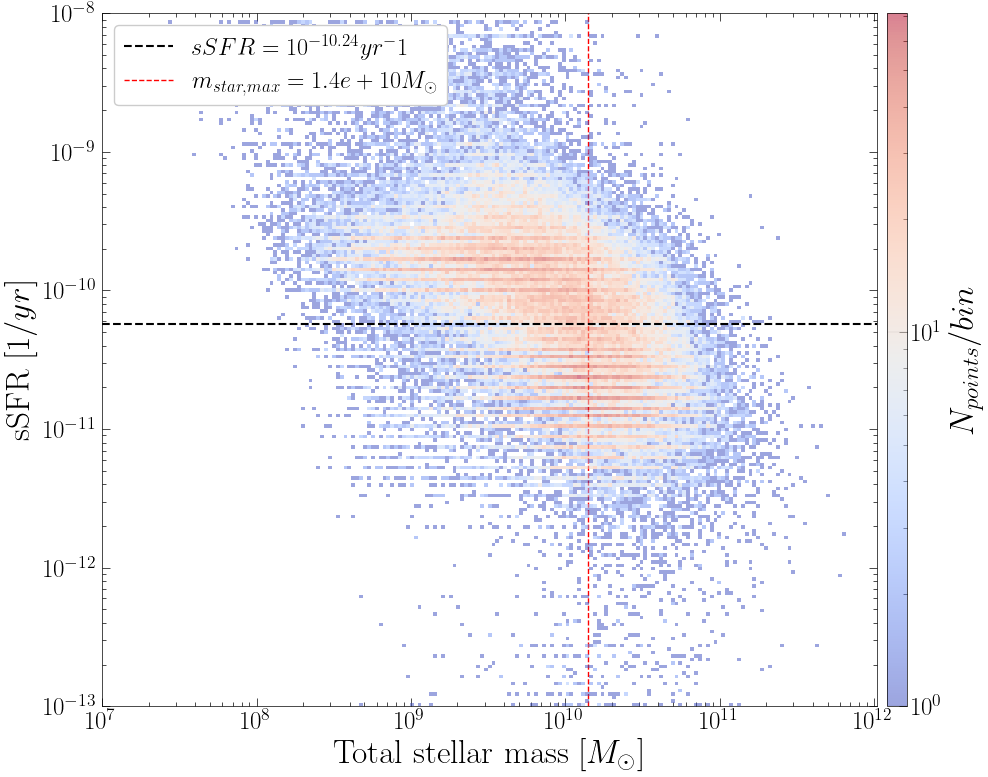
\includegraphics[width=0.86\columnwidth]{images/sSFRvsmstar.png}
    \caption{sSFR versus $m_\text{star}$ scatter-plot. The black dashed line separates the main sequence from passive galaxies. The red dashed line indicates $m_\text{star,max}$, that is the stellar mass corresponding to the upper limit in the halo mass for which we have effective cooling. The colour indicates the density of galaxies in the region of the plot.}
    \label{fig:sSFR_mass}
\end{figure}


We assume that the gas content drives star formation with its collapse; one can model its evolution with:


\begin{equation}
\dfrac{dm_\text{gas}(t)}{dt} , = , \dot{m}\text{gas}^\text{in}(t) - \dot{m}\text{gas}^\text{out}(t) - \left(1-R\right)\text{SFR}(t),
\label{eq:dmgas_dt_old}
\end{equation}


with $\dot{m}\text{gas}^\text{in}(t)$  the rate at which gas flows into the galaxy, $\dot{m}\text{gas}^\text{out}(t)$ is the rate of gas outflow, and $R$ is the fraction of gas that returns to the interstellar medium after participating in star formation, through processes such as supernovae and stellar winds.\\

We can connect the gas mass of a galaxy to its star formation rate using the Kennicutt-Schmidt empirical law (\cite{Kennicutt_Jr_1998}), which relates the surface density of gas to the surface density of star formation. In our simplified model, we express this relationship as:

\begin{equation}
\text{SFR}\left(m_\text{gas}\right) \simeq \dfrac{\epsilon}{\tau_\text{dyn}} m_\text{gas} \doteq \epsilon' m_\text{gas},
\label{eq:SFR_vs_gasmas}
\end{equation}

With $\epsilon \simeq 0.02$ an efficiency parameter. 
$\tau_\text{dyn}$ is the dynamical time of the galaxy, given by:


\begin{equation}
\tau_\text{dyn} = 2 \times 10^7 \text{yr} \left(\dfrac{R_{1\slash2}}{4\text{kpc}}\right) \left(\dfrac{v_\text{circ}}{200\text{km s}^{-1}}\right)^{-1}.\\
\label{eq:t_dynamical}
\end{equation}


where $R_{1/2}$ is the half-light radius of the galaxy and $v_\text{circ}$ is the circular velocity. In our model, we assumed a constant $\tau_\text{dyn} = 2 \times 10^7 \text{yr}$.

%%%%%%%%%%%%%%%%%%%%%%%%%%%%%%%%%%%%%%%%%%%%%%%%%

\subsubsection{\textbf{Gas outflow: $\dot{m}_\text{gas}^\text{out}(t)$}}
\label{gas_out}
Gas outflow from galaxies can occur through several mechanisms. Supernovae, both Type Ia and Type II, inject energy into the interstellar medium, expelling gas. There can be AGN feedback, that becomes more significant in galaxies with larger black holes. In clusters, ram pressure stripping can also remove gas as galaxies move through the hot intracluster medium.

For our model, we assume Type IIa supernovae to be the dominant mechanism driving gas outflows, given their frequency in star-forming regions and the big energy they release. We can model their outflow rate as:

\begin{equation}
    \dot{m}_\text{gas}^\text{out}(t) \, \simeq \, \eta\text{SFR}(t),\\
	\label{eq:mgas_outflow}
\end{equation}
where $\eta$ is the mass-loading factor representing the efficiency of stellar feedback in driving outflows.\\

Eq. (\ref{eq:dmgas_dt_old}) becomes:

\begin{equation}
    \dfrac{dm_\text{gas}(t)}{dt} \, = \, \dot{m}_\text{gas}^\text{in}(t) - \left(1+\eta-R\right) \dfrac{\epsilon}{\tau_\text{dyn}} m_\text{gas}.
	\label{eq:dmgas_dt}
\end{equation}


\subsubsection{\textbf{Gas inflow : $\dot{m}_\text{gas}^\text{in}(t)$}}

The gas inflow into a galaxy is connected to the properties of its surrounding dark matter halo. We can express this relationship as:

\begin{equation}
\dot{m}_\text{gas}^\text{in}(t) = \xi \dot{m}_\text{halo,\rm gas}^\text{in}(t) = \xi f_\text{gas} \dot{m}_\text{halo}^\text{in}(t),\\
\label{eq:mgas_inflow}
\end{equation}

Where we assume $f_\text{gas}=0.15$, representing the baryon fraction, and $\xi \in [0,1]$ is a function related to the cooling efficiency of the gas.\\
To determine $\dot{m}_\text{halo}^\text{in}$, we rely on results from the Millennium Simulation (\cite{10.1111/j.1365-2966.2009.15329.x}, which provides:
{\fontsize{7.9pt}{7.9pt}\begin{equation}
\dot{m}_\text{halo}^\text{in}(z) = 42 M_{\odot} \text{yr}^{-1} \left(\dfrac{m_\text{halo}}{10^{12}M_{\odot}}\right)^{1.127} (1+1.17z) \sqrt{(1+z)^3 \Omega_m + \Omega_\Lambda},
\label{eq:mcbride}
\end{equation}}
where we adopt $\Omega_m=0.3$ and $\Omega_\Lambda=0.7$ for the cosmological parameters.

However, this requires knowledge of $m_\text{halo}$, which isn't directly observable from our photometric data. To overcome this, we use the empirical relation from \cite{moster_2012} to link stellar mass to halo mass:
{\fontsize{9pt}{9pt}\begin{equation}
m_\text{star} \left(m_\text{halo}\right) = 2N m_\text{halo} \left[\left(\dfrac{m_\text{halo}}{M_1}\right)^{-\beta} + \left(\dfrac{m_\text{halo}}{M_1}\right)^\gamma\right]^{-1},
\label{eq:moster}
\end{equation}}
where $\beta$, $\gamma$, M and N are parameters that depend on redshift, they can be found in \cite{moster_2012}, we use their value for our sample's mean redshift $z_{\text{mean}} \approx 0.054$.\\

By inverting this relation numerically, we can estimate $m_\text{halo}$ in function of the stellar mass and therefore compute $\dot{m}_\text{in}(m_\text{star})$

\subsubsection{\textbf{Cooling}}

The efficiency of gas cooling plays a crucial role in galaxy formation. For gas to infall and form structures, the cooling time must be shorter than the free-fall time (the time scale on which the gas responds to gravitational forces): $\tau_{\text{cooling}} < \tau_{\text{free-fall}}$ .
This condition can be translated into constraints on halo mass (see chapter 8.4 of \cite{Mo_van}).
To have effective cooling one needs:

\begin{equation}
m_{\text{halo}} \in \left( m_{\text{halo,min}}=10^9 M_\odot , m_{\text{halo,max}}=10^{11.6} M_\odot \right),
\label{eq:halo_mass_minmax}
\end{equation}

Using the \cite{moster_2012} relation, we can translate these halo mass limits into stellar mass limits:

\begin{equation}
m_\text{star} \in \left( m_\text{star,min}=10^{4.3} m_\odot, m_\text{star,max}=10^{10.1} M_\odot \right).
\label{eq:star_mass_minmax}
\end{equation}


In our catalogue, we observe that the most massive galaxies exceed $M_\text{star,max}$ (see Fig. \ref{fig:sSFR_mass} and Fig. \ref{fig:frac_MS}), suggesting they don't have efficient cooling ($\xi \simeq 0$) and consequently ($\dot{m}_\text{gas}^\text{in} \simeq 0$). This observation allows us to divide our galaxies into two distinct populations, which we can model using different simplifying assumptions. We'll connect the two models with a sharp transition at $m_\text{star,max}$. 


\begin{figure}\centering
	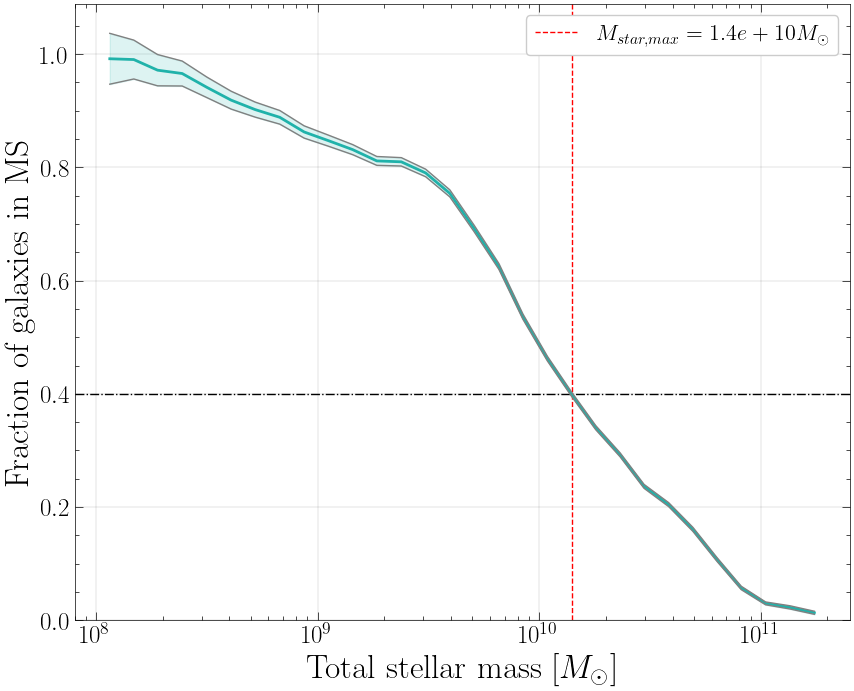
\includegraphics[width=0.86\columnwidth]{images/Frac_MS_mass.png}
    \caption{Fraction of galaxies on the Main Sequence in function of their stellar mass. The red dashed line indicates $m_\text{star,max}$, that is the stellar mass corresponding to the upper limit in the halo mass for which we have effective cooling. The black dashed line indicates the point in which 60\% of the galaxies are in the passive region.}
    \label{fig:frac_MS}
\end{figure}

Massive (and therefore passive) galaxies may be approximated with a closed-box model, assuming no gas exchange with their surroundings. In contrast, star-forming galaxies require an open-box model, accounting for both gas accretion and ejection.


\subsection{Models}
\label{models} % used for referring to this section from elsewhere

\subsubsection{\textbf{Closed box}}
The simplest model we can write is the one for passive galaxies, where we assume there is no inflow and outflow of gas (closed box: $\dot{m}_\text{gas}^\text{in}=0$ and $\eta=0$). This assumption leads to a straightforward solution for the gas mass evolution (Eq. (\ref{eq:dmgas_dt}) ):

{\fontsize{9pt}{9pt}\begin{equation}
m_\text{gas}(t) = m_\text{gas}(t_0)e^{-(1-R)\epsilon' (t-t_0)},\\
	\label{eq:mgas_closedbox}
\end{equation}}
with $m_\text{gas}(t_0)$ the initial gas resevoir.\\

The sSFR would become:

\begin{equation}
    sSFR(t) = \frac{\epsilon' m_\text{gas}(t)}{m_\text{{star}}} = \frac{m_\text{gas}(t_0)e^{-(1-R)\epsilon' (t-t_0)}}{m_\text{{star}}}.\\
    \label{eq:sSFR_closed}
\end{equation}

To test our model with data we need the sSFR in function of stellar mass, so we have to make another simplifying assumption: galaxies accrete their halo mass at a constant rate. This way one can write: 

\begin{equation}
   \Delta t = \frac{m_\text{halo}(t)- m_\text{halo}(t_0)}{\dot{m}_\text{halo}}. \\
   \label{eq:deltat}
\end{equation}

Inverting Eq. (\ref{eq:moster}) we can get $m_\text{halo}(m_\text{star})$ and therefore compute the $sSFR(m_\text{star})$ putting $\Delta t$ from Eq. (\ref{eq:deltat}) in  Eq. (\ref{eq:sSFR_closed}).


\subsubsection{\textbf{Open box}}
For galaxies in the star-forming region, (or Main Sequence), we can make a different simplifying assumption: in these galaxies we consider the inflow and outflow of gas to be balanced. This equilibrium condition leads to a different expression for the gas mass evolution( Eq.
(\ref{eq:dmgas_dt})):

{\fontsize{7.9pt}{7.9pt}\begin{equation}
    m^\text{eq}_\text{gas}(t) = \dfrac{\dot{m}_\text{gas}^\text{in}(t)}{(1+\eta-R)\epsilon'} \: \Rightarrow \: sSFR^\text{eq}\left(m_{\text{star}}\right) = \dfrac{\dot{m}_\text{gas}^\text{in}\left(m_{\text{star}}\right)}{1+\eta-R} \, \dfrac{1}{m_\text{star}},
	\label{eq:openbox_equilibrium}
\end{equation}}

where $\dot{m}_\text{gas}^\text{in}\left(m_{\text{star}}\right)$ is determined equations (\ref{eq:mgas_inflow}), (\ref{eq:mcbride}), and (\ref{eq:moster}), using our sample's mean redshift of $z_\text{mean} \approx 0.054$. We keep $\eta$ and $R$ as free parameters of the model. 

\subsubsection{\textbf{Open box for MS galaxies and closed box for passive ones}}
We then implement a mixed approach that combines our open-box model for main sequence galaxies with a closed-box model for passive galaxies.\\
We impose a sharp transition between these two regimes at the maximum halo mass for which efficient cooling occurs $m_\text{star, max}$. This transition point corresponds to a halo mass of $10^{11.6} M_\odot$ and a stellar mass of approximately $10^{10.15} M_\odot$, shown by the red dotted line in Fig. \ref{fig:mixed_open_closed}.
Connecting these two models some parameter tuning is needed to represent the observed data accurately. 
In the closed box model we set:
\begin{enumerate}
    \item the gas recycling fraction (R) to the same value used in the open-box model, to keep consistency,
    \item $m_\text{star}(t_0)$ =  $m_\text{star, max}$
    \item $\epsilon = 0.01$
    \item $m_\text{gas}(t_0)$ since we don't know it, is treated as a free parameter, to match the two behaviours.
\end{enumerate}

In Fig. \ref{fig:mixed_open_closed} the open box model is shown with a solid red line, we plot it only for masses smaller than $m_\text{star, max}$. The solid blue line shows the sSFR-$m_\text{star}$ relationship for the closed box.


\begin{figure}\centering
	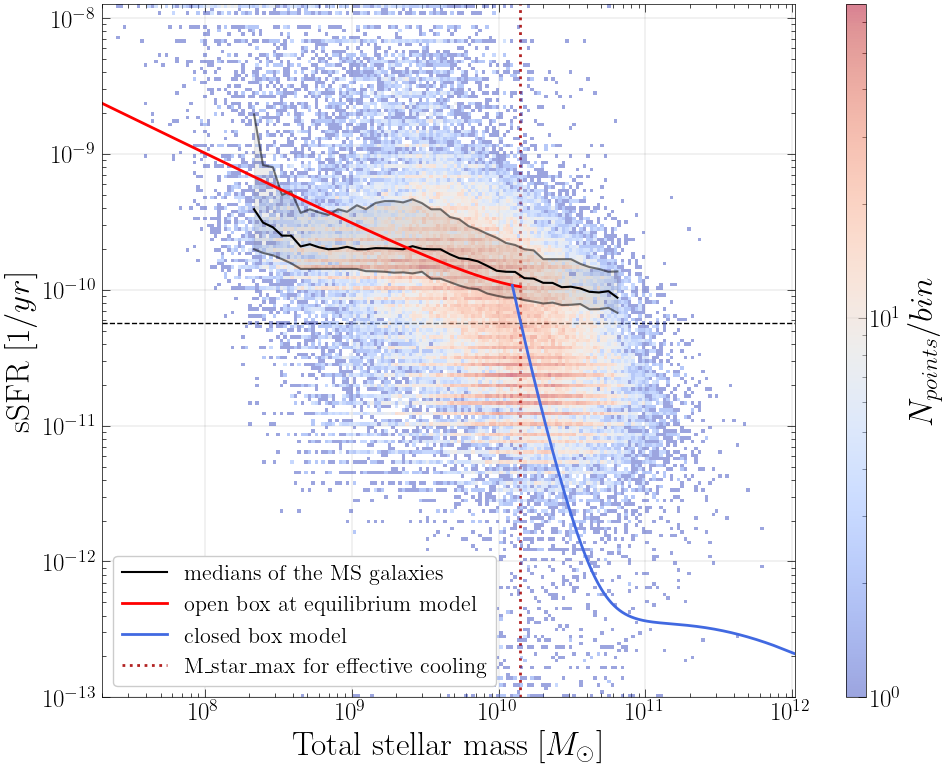
\includegraphics[width=0.86\columnwidth]{images/sSFR_mass_due_andamenti.png}
    \caption{sSFR versus $m_\text{star}$ scatter-plot.
    The red and blue solid lines show the sSFR vs stellar mass relation respectively in the open and closed box models.
    The black solid line is the median of the main sequence, the black dashed line separates the main sequence from passive galaxies. The red dashed line indicates $m_\text{star,max}$, that is the stellar mass corresponding to the upper limit in the halo mass for which we have effective cooling. The colour indicates the density of galaxies in the region of the plot.}
    \label{fig:mixed_open_closed}
\end{figure}

%%%%%%%%%%%%%%%%%%%%%%%%%%%%%%%%%%%%%%%%%%%%%%%%%%%%%%%%%%%%%%%%%%%%%%%%%%%%

\subsubsection{\textbf{Numerical model}}

A numerical approach allows us to integrate the gas mass evolution equation (Eq.(\ref{eq:dmgas_dt})) over small time steps, from galaxy formation to observation.\\
The different evolution of the galaxies is only driven by the different formation times $t_\text{form,i} \in \left( 0.1, 1 \right) Gyr$, in fact they all start with an initial halo mass of $5 \times 10^8 M_\odot$.\\
At each timestep of 10 Myr we evaluate halo mass ($m_\text{halo}$), gas mass ($m_\text{gas}$), star formation rate (SFR), and  stellar mass ($m_\text{star}$, time integral of the SFR), using equations (\ref{eq:dmgas_dt}), (\ref{eq:mgas_inflow}), (\ref{eq:mcbride}), and (\ref{eq:SFR_vs_gasmas}). We also take into account the redshift dependencies in ($\dot{m}_\text{gas}^\text{in}$) and ($\tau_\text{dyn}$), that we were neglecting in the two previous models.

When a galaxy forms earlier, it reaches the minimum halo mass required for efficient cooling sooner (\ref{eq:halo_mass_minmax}). At this point, star formation begins, and the galaxy enters a period of equilibrium between gas inflow and outflow, and it's located on the main sequence.
As the halo continues to grow, it eventually reaches its maximum mass for efficient cooling: the gas content decreases exponentially and the galaxy becomes passive.

This understanding is supported by the data showing that passive galaxies are, on average, older than star-forming galaxies (see Fig. \ref{fig:mass_sSFR_age}).

\begin{figure}\centering
	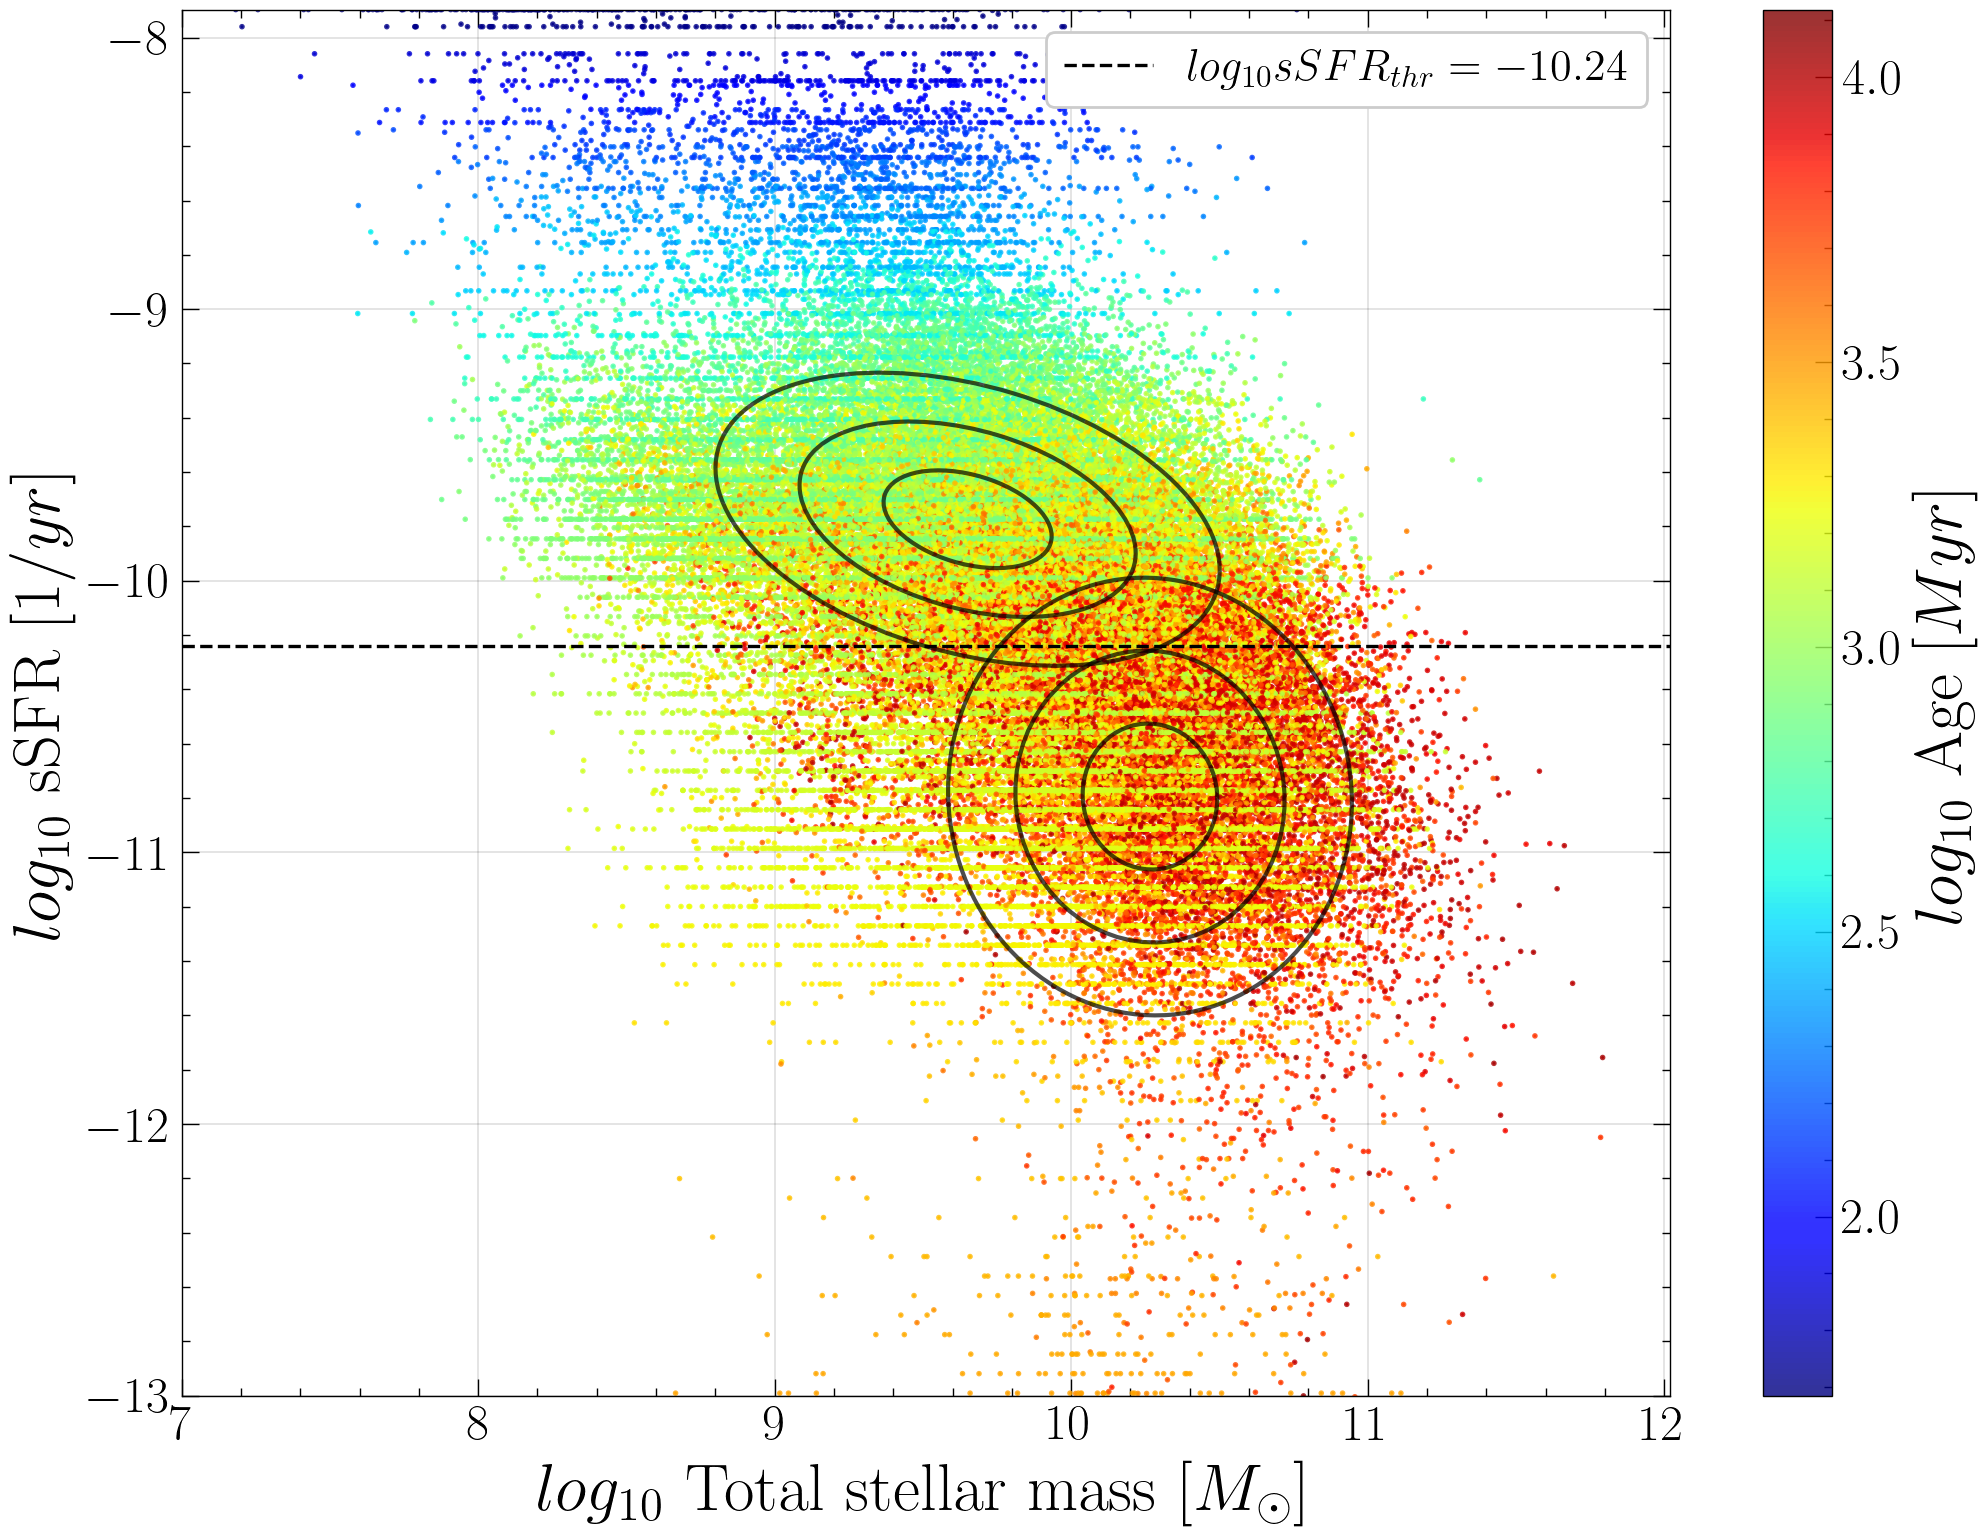
\includegraphics[width=0.86\columnwidth]{images/sSFR_Mass_AgeColormap.png}
    \caption{sSFR versus $m_\text{star}$ scatter-plot, the black dashed line separates the main sequence from passive galaxies. The red dashed line indicates $m_\text{star,max}$. The colour is proportional to the age of the galaxy.}
    \label{fig:mass_sSFR_age}
\end{figure}
%%%%%%%%%%%%%%%%%%%%%%%



The cooling efficiency function $\xi$ in Eq. (\ref{eq:mgas_inflow}) determines the transition between the star-forming and passive regimes. We explore two options for this function:

A step function, representing a sharp transition in cooling efficiency, as soon as the maximum mass for effective cooling is reached: 
\begin{align}
    \xi_\text{step} &= 1 \:\:\:\: \text{if} \:\:\:\: m_{\text{halo}} \in \left( m_{\text{halo,min}} \, , \, m_{\text{halo,max}} \right) \\
    \xi_\text{step} &= 0 \:\:\:\: \text{if} \:\:\:\:m_{\text{halo}} \notin \left( m_{\text{halo,min}} \, , \, m_{\text{halo,max}} \right)
    \label{eq:xi_step}
\end{align}
 

A more complex model proposed by Davé et al. (2011) (\cite{dave_analytic_2012}) , accounting for various physical processes affecting gas accretion (photoionization heating, SMBH quenching, gravitational heating, and wind effects):
\begin{equation}
\xi_\text{Davé} = \xi_\text{photo} \cdot \xi_\text{quench} \cdot \xi_\text{grav} \cdot \xi_\text{winds}\\
\label{eq:xi_dave}
\end{equation}

The $\xi_\text{Davé}$ function provides a smoother transition than $\xi_\text{step}$ and better fits our data (Fig. \ref{fig:numerical_dave}).

\begin{figure}\centering
	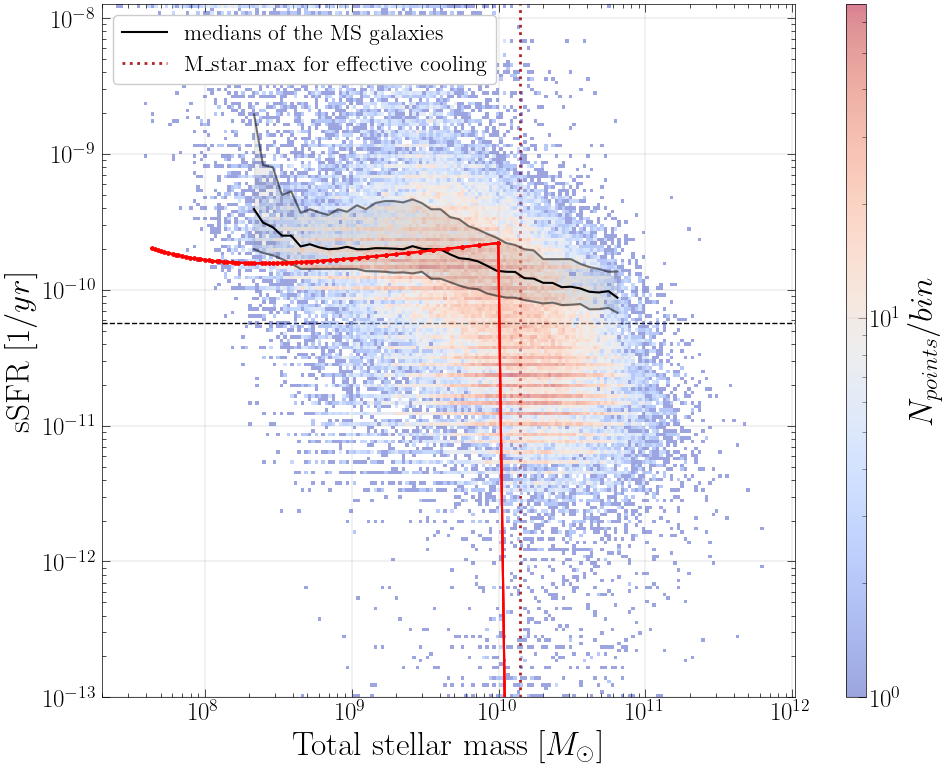
\includegraphics[width=0.86\columnwidth]{images/sSFR_mass_Cantacode_csi_old_5-5.png}
    \caption{sSFR versus $m_\text{star}$ scatter-plot. The red line is the numerical relation for specific star formation rate (sSFR) versus stellar mass ($M_\text{star}$) at the observation time, for galaxies with different formation times. In this case we used a step function for the cooling efficiency function $\xi$.
    The black solid line is the median of the main sequence, the black dashed line separates the main sequence from passive galaxies. The red dashed line indicates $m_\text{star,max}$.}
    \label{fig:numerical_step}
\end{figure}

\begin{figure}\centering
	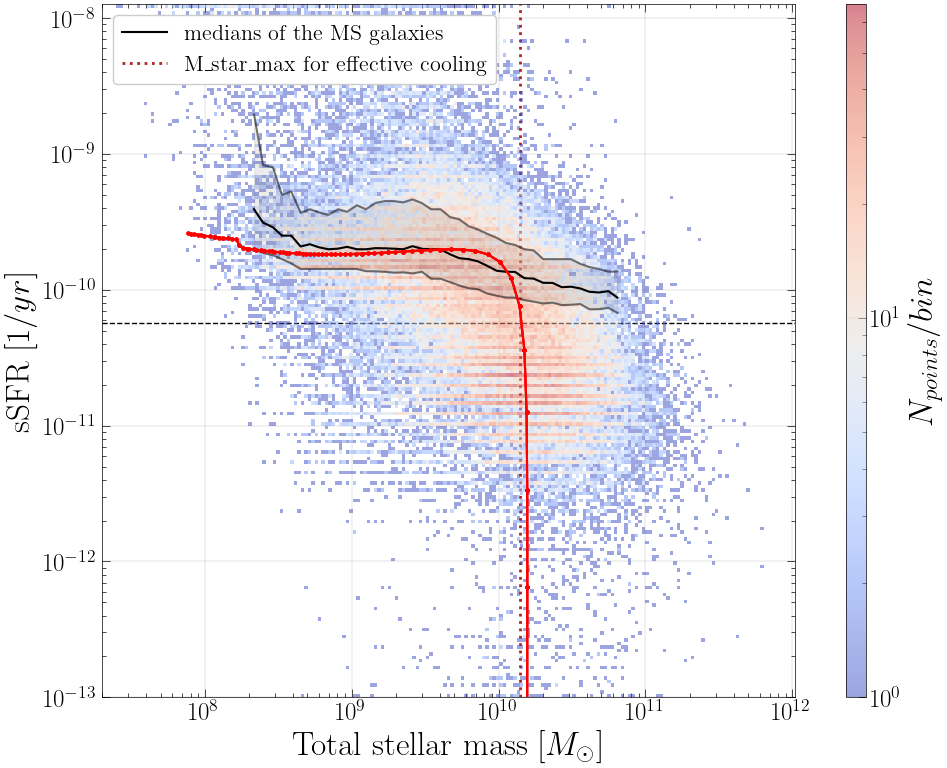
\includegraphics[width=0.86\columnwidth]{images/sSFR_mass_Cantacode_csi_Dave.png}
    \caption{sSFR versus $m_\text{star}$ scatter-plot. The red line is the numerical relation for specific star formation rate (sSFR) versus stellar mass ($M_\text{star}$) at the observation time, for galaxies with different formation times. In this case we used a Davè's function for $\xi$.
    The black solid line is the median of the main sequence, the black dashed line separates the main sequence from passive galaxies. The red dashed line indicates $m_\text{star,max}$. }
    \label{fig:numerical_dave}
\end{figure}


Figures \ref{fig:numerical_step} and \ref{fig:numerical_dave} show the specific star formation rate (sSFR) versus stellar mass ($M_\text{star}$) at the observation time for galaxies with different formation times, using the step function and Davé models, respectively.
To match observational data, we had to scale the absolute magnitudes of sSFR. For the step function model, we used $\eta=4$ and $R=0.1$, with a vertical offset correction factor of $\simeq
4$. The Davé model required $\eta=1.3$ and $R=0.4$, with a correction factor of $\simeq 7$.



\section{Discussion}

Both the model that differentiates between star-forming and passive galaxies, and our numerical time-evolution model, successfully capture the observed trends: a relatively constant specific star formation rate (sSFR) for Main Sequence (MS) galaxies and a drop for passive galaxies.\\

In the open-box model, we assumed an equilibrium between gas inflow and outflow. However, this assumption may not hold everywhere, in particular for low-mass galaxies. These younger systems may not have reached equilibrium yet, which could explain why our model less accurately describes their behavior.

The closed-box model, with its assumption of no gas exchange, is likely an oversimplification. While it helps simplify our calculations, it may be too restrictive.\\
Moreover the slope of the sSFR-$m_\text{star}$ relation dependends heavily on parameters we adjusted to fit the observed behavior, suggesting there might be additional processes that we haven't accounted for.

Our numerical implementation offers a more general approach by avoiding assumptions about equilibrium and allowing inflow and outflow rates to evolve naturally. It also accounts for the mass-loading factor ($\eta$) in the passive region.

However, the numerical model is not without its challenges. While it successfully reproduces the overall shape of both the star-forming main sequence and the passive galaxy distribution, we have to apply scaling factors to match the observed magnitudes. This need for manual adjustment suggests that our model, even if it captures the key trends, may be missing some  processes or factors influencing galaxy evolution.

These limitations underscore the complexity of galaxy evolution and challenges in developing models that can describe it fully.

We could improve our description by accounting for different processes in the outflow (see  section \ref{gas_out}) such as AGN feedback (proportional to the mass of the BH) and ram pressure stripping. 
One should also consider the environment in which the galaxy lives in, to account for interactions with other galaxies or with the hot gas of the Intra Cluster Medium.

\section{Summary}

Our study focused on analyzing a subset of the Sloan Digital Sky Survey (SDSS) catalog and extract from it crucial information about galaxies through fitting various model combinations using the CIGALE software. 
The key observation from our analysis was the bimodality in the specific star formation rate (sSFR) versus stellar mass plot, showing two distinct galaxy populations: star-forming and passive.
To model these populations, we developed two main approaches:

We distinguished between star-forming and passive galaxies, applying different simplifying assumptions to each population. This allowed us to adjust our models to the specific characteristics of each group, capturing their different evolutions.

We implemented a time-dependent numerical calculation of galaxy properties, assuming that the primary driver of evolutionary differences is galaxy age. This model considers how halo mass increases over time and determines whether gas can cool efficiently to form structures.

Both models successfully captured the key trends observed in our data, however, achieving this required quite a lot of fine-tuning of model parameters. Notably, in the numerical model, we needed to adjust the overall magnitude of the sSFR to match observed data.

We can reproduce the broad trends, but the need for parameter tuning and magnitude adjustments suggests that there are still aspects of galaxy evolution that our models do not capture fully.

%%%%%%%%%%%%%%%%%%%% REFERENCES %%%%%%%%%%%%%%%%%%

% The best way to enter references is to use BibTeX:

\bibliographystyle{mnras}
\bibliography{report} % if your bibtex file is called example.bib



% Don't change these lines
\bsp	% typesetting comment
\label{lastpage}
\end{document}

% End of mnras_template.tex
